\documentclass[hyperref]{ctexart}
\usepackage[left=2.50cm, right=2.50cm, top=2.50cm, bottom=2.50cm]{geometry} %页边距
\usepackage{helvet}
\usepackage{amsmath, amsfonts, amssymb} % 数学公式、符号
\usepackage[english]{babel}
\usepackage{graphicx}   % 图片
\usepackage{url}        % 超链接
\usepackage{bm}         % 加粗方程字体
\usepackage{multirow}
\usepackage{booktabs}
\usepackage{algorithm}
\usepackage{algorithmic}
\usepackage{fancyhdr} %设置页眉、页脚
\pagestyle{fancy}
\lhead{}
\chead{}
\lfoot{}
\cfoot{}
\rfoot{}
\usepackage{hyperref} %bookmarks
\hypersetup{colorlinks, bookmarks, unicode} %unicode
\usepackage{multicol}
\title{\textbf{穆斯堡尔效应实验}}
\author{\sffamily 赵宇航}
\date{}
\begin{document}
\maketitle
\indent{\bf 摘要: }本实验通过测量$\alpha-Fe$的穆斯堡尔谱,验证了Fe的超精细结构,并分析了放射源的选取和一些实验器材的作用。\\	
\begin{multicols}{2}
\CTEXsetup[format={\Large\bfseries}]{section}
	\section{实验目的}
	1.学习并掌握穆斯堡尔效应的原理;

	2.了解、熟悉穆斯堡尔谱仪的结构和工作原理;

	3.了解并掌握通过测量穆斯堡尔谱获取物质超精细参数的方法。
	\section{实验原理}
	
	\subsection{$\gamma$射线与穆斯堡尔效应}
	\subsubsection{$\gamma$射线的产生与谱线的自然线宽}
	$\gamma$射线是波长极短的电磁波。和原子类似,原子核也可以处与不同的能量状态,即我们常说的能级。当不稳定的原子核从具有较高能量的激发态能级跃迁到较低能级(例如基态)时,就会放射出$\gamma$射线。反之,如果原子核可以吸收具有某一个特定能量的$\gamma$射线,则可以从一个较低的能量状态跃迁回到一个较高能量状态。
	
	由于原子核的激发态存在有限长的寿命τ,则它跃迁后发射的$\gamma$射线能量不是唯一值,表现为能量谱线具有洛伦兹分布,而且对应的能量谱线具有一定宽度。已知光子的能量谱线强度和光子频率ω之间的关系是
	\begin{equation}
	I(\omega)\propto \frac{1}{(\omega-\omega_0)^2+(\frac{1}{2\tau})^2}
	\end{equation}
	
	考虑到光子的能量$E=h\omega$ (h 为约化普朗克常数),得到谱线强度按照能量的分布:
	\begin{equation}
	I(E)\propto \frac{1}{(\omega-\omega_0)^2+(\frac{1}{2\tau})^2}
	\end{equation}
	当 $E-E_0=\pm\frac{h}{2\tau}$ 时,可以计算出谱线的强度下降为最大值的一半。这时我们可以将对应的谱线半高宽称为$\gamma$射线的自然线宽$\Gamma$。而且根据海森堡的测不准关系易知τ和$\Gamma$满足:
	\begin{equation}
	\Gamma\sim \frac{h}{\tau}\label{kd}
	\end{equation}
	
	\begin{center}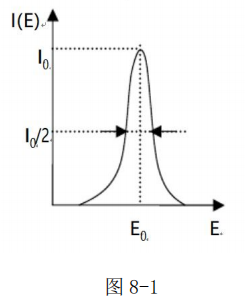
\includegraphics[scale=0.5]{t81.png}\end{center}
	图 8-1 为典型的洛伦兹型吸收谱线,线宽为$\Gamma$ 。而对于发射谱线和吸收谱线均具有类似上式的能量分布
	\begin{equation}
	I(E)\propto \frac{1}{(E-E_0)^2+(\frac{1}{2\Gamma})^2}
	\end{equation}
	
	\subsubsection{原子核对$\gamma$射线的有反冲共振吸收现象}
	正如前面所述,原子核中由高到低的能级跃迁可以放出$\gamma$射线,反之如果能够吸收合适能量的$\gamma$射线,也可以从低能级跃迁到高能级。这种不同能量状态之间的跃迁就是我们熟悉的$\gamma$辐射和$\gamma$吸收现象。考虑到原子核的质量比较小,而放射或者吸收的$\gamma$射线的能量又比较大(通常在 keV 到 MeV 量级),因此在放射和吸收过程中必须要考虑到原子核的反冲现象对放射和吸收谱线的影响。假设原子核的质量为m ,初速度为零,激发态$E_e$ 和基态$E_g$ 的能级差为$E_0=E_e-E_g$ ,辐射$\gamma$射线时为了保证动量守恒,原子核的反冲动量$mu_R$ 应该等于发射$\gamma$射线的动量$P_y$ ,即$mu_R=P_y =\frac{E_y}{c}$。根据能量守恒定律:$E_0 =E_y+ E_R$ ,可得原子核的反冲动能$E_R$因此原子核反冲会导致实际发射的 $\gamma$ 射线能量为$E_0-E_R =(E_e + E_g)-E_R$ ,小于能级差$E_0$,而消耗的能量在原子核的反冲动能 $E_R$上。反正在原子核的共振吸收时也会碰到同样的现象:如果需要从基态跃迁到激发态,$\gamma$射线所需要提供的能量为($E_e$-$E_g$ )+$E_R$ ,多出的能量使共振原子核有一个反冲能 $E_R$ 。

	因此发射谱和吸收谱就会产生 2 $E_R$ 的偏移,如图 8-2(a)所示。这个反冲能能量 $E_R$ 与原子核的质量和$\gamma$射线的能量有关,在某些特定情况下比自然线宽$\Gamma$大得多,以我们实验中用的$^{57}Fe$ 原子核为例,E0=14.41keV,则 $E_R\approx2\times{10}^{-3}$eV, 而对应的自然线宽为 ${10}^{-8}$eV 量级,因此造成吸收谱和发射谱之间的重叠很少,应该看不到共振吸收现象。在上面的讨论中,我们假设原子是孤立的、自由的和静止的。实际情况是原子核有热运动,因此也会由热运动提供一定的多普勒能量,使发射谱和吸收谱有很大展宽,而不等于自然线宽,这种谱线的增宽称为多普勒增宽,展宽后的谱线宽度为$E_d=2\sqrt{E_K E_R}$ ,其中$E_K=\frac{K_BT}{2}$ 为一个原子核每个自由度平均动能。图 8-2(b)中的$E_d$大约在 ${10}^{-2}$eV 的量级,这样会使吸收和发射谱线可能会有一定的重叠。所以原则上讲,可以通过提高测量温度是原子核热运动加快,产生较多的谱线重叠,以获得有反冲的原子核对$\gamma$射线的共振吸收。在发现穆斯堡尔效应之前,通常使用的办法主要就是采用加热和加速的办法补偿反冲时的能量损失,而且由于总的重叠面积较小,要想观察这种原子核的有反冲共振吸收总是比较困难。

	\begin{center}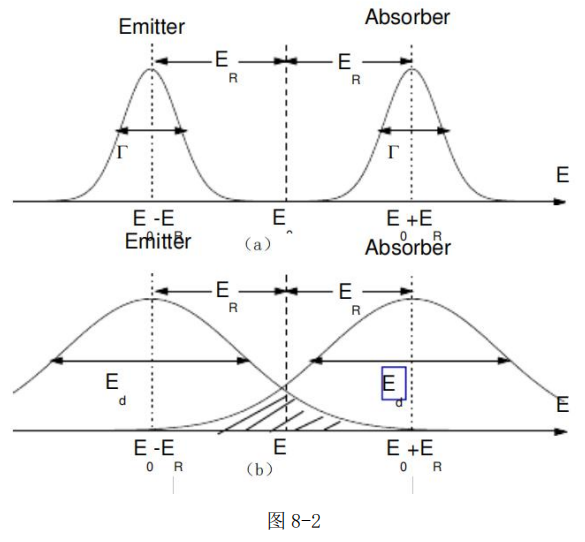
\includegraphics[scale=0.3]{t82.png}\end{center}
	\subsubsection{原子核对$\gamma$射线的无反冲共振吸收现象(穆斯堡尔效应)}
	前面考虑的均为有反冲共振吸收现象,那么如果有一种办法可以使原子核被牢牢固定,应该可以减小反冲能 Ed ,甚至使之趋向于零,这样发射谱线和吸收谱线的叠加将明显增加,共振效应也易观察到。具体讲来,如果把发射核和吸收核均牢牢地固定在固体晶格中,当发射或吸收$\gamma$射线时,需要考虑的反冲能$E_R=\frac{E_\gamma^2}{2Mc^2}$,其中 M 为晶体的质量,远远大于单个原子核的质量 m,因此反冲能急剧减小,甚至可以看为 0。这样发射谱线和吸收谱线可以认为完全重合,可以获得非常大的重合面积,很容易发生共振吸收现象。但是实际上的过程比前面所说的要复杂的多,因为晶格的振动是一种量子化的体系,根据爱因斯坦模型如果提供$h\omega,2 h\omega,3 h\omega$等能量就可以改变晶格的振动状态,即激发出声子,声子的频率为$\omega$ 。如果在这个过程中不产生或者吸收声子,那么发射和吸收$\gamma$射线的能量就不会改变,因此原子核不会产生反冲能量损耗。这种没有反冲能量损耗的$\gamma$射线发射或者吸收过程的概率就被称为无反冲分数 f。实际上爱因斯坦模型过于简单,更接近实际的是晶格振动的德拜模型,但仍然可以获得类似结果。所以一句话来说,穆斯堡尔效应就是原子核对$\gamma$射线的零声子无反冲共振和吸收效应。

	在晶格振动的爱因斯坦模型下,可计算出固体中有关和产生穆斯堡尔效应的几率即无反冲分数$f=exp[-\frac{E_y^2<x^2>}{(hc)^2}]$,实际是固体中的穆斯堡尔核在发
射或吸收$\gamma$光子时不激发或吸收声子(零声子)过程的几率,又被称为穆斯堡尔分数。其中$<x^2>$ 为穆斯堡尔原子在$\gamma$射线传播方向上的均方振幅。要易于观察到穆斯堡尔效应,f 必须尽可能的大,这就要求$\gamma$光子的能量不能太高(低能的$\gamma$辐射),穆斯堡尔原子与基质原子间的束缚要强,实验温度不能太高(这点恰好和原子核的有反冲共振吸收的实验现象相反,也正是穆斯堡尔发现这个效应的根源)。此式表明:在液体、气体中,因$<x^2>$ 很大,以至难以观察到穆斯堡尔效应。当然并不是发射核或吸收核只要存在于固体之中就必定发生穆斯堡尔效应,但只有在固体之中的核才有可能产生穆斯堡尔效应。凡有穆斯堡尔效应的原子核我们称之为穆斯堡尔核。

	例如,在室温下$^{57}Fe$ 的无反冲分数可高达 0.7-0.8。此外$^{119}Sn$的 23.87 keV的$\gamma$跃迁在室温下有较大的无反冲分数,这两者是应用最为广泛的穆斯堡尔核。而目前发现的有穆斯堡尔效应的 43 种元素,80 多种同位素的 100 多个核跃迁大多数需要在低温下才能观察到,因此使用并不广泛。

	在无反冲共振吸收时,$\gamma$射线的能量宽度为激发态的自然宽度,测得的穆斯堡尔谱线的宽度近似等于谱线的自然宽度,其值一般是相当小的。仍然以$^{57}Fe$(14.41 keV)为例,$\Gamma\sim-4.6\times{10}^{-9}$ eV,而$\frac{\Gamma}{E_\gamma}\sim -3.2\times{10}^{-13}$,这就是通常所说的穆斯堡尔谱的能量分辨率。因此可以看出,这种方法具有很高的能量分辨率。如果原子核的能级由于某种原因有非常细小的变化,也可能会使我们无法观测到无反冲共振吸收现象,这样我们可以通过观察谱线的移动测量相应的能级移动。所以说穆斯堡尔效应的发现,不仅仅使我们能够很容易的观察到核的共振吸收现象,更重要的是我们能够利用它的高能量分辨率特性来研究原子核的超精细结构。

	\subsubsection{多普勒效应和穆斯堡尔谱}
	一个光源发射的光子频率为ω,当它以速度 V 向观察者移动时,即发射光子的方向和 V 的方向一致,则观察者接收到的光子频率有一个增加,而且满足$\frac{\triangle \omega}{\omega}=\frac{V}{c}$ 。如果 V 和发射$\gamma$光子的方向有一个夹角$\theta$则吸收体接收到$\gamma$射线的能量存在一个移动为$E_d=\frac{v}{c}E_y\cos{\theta}$,而这时候发射出的$\gamma$射线的能量为$E_y=E_0-E_R+E_d$。

	在前面原子核的有反冲共振吸收中谈过的多普勒热展宽也是由于多普勒效应的影响。为了简单估算多普勒热展宽的大小和它的影响,我们可以假定晶格振动能量的均分定理近似成立,这时晶格在某一方向的平均热运动能量为$E_K=\frac{1}{2}m{\overline{V}}^2=\frac{1}{2}K_BT$,其中 $K_B$ 为玻耳兹曼常数,方均根速度$\overline{V}=(\frac{K_BT}{m})^{\frac 1 2}$则此时处与晶格位置的原子核发射的$\gamma$射线能量$E_\gamma$ 存在一个多普勒展宽为,计算出的$^{57}Fe$ 在 T=300K 时的$E_d =2\times{10}^{-2}$eV。

	对于无反冲共振吸收而言,反冲能$E_R$可以认为等于零,那么发射出的$\gamma$射线的能量可以简单地通过改变放射源的运动速度来控制。放射源所附加的多普勒速度为$E_d =
\frac{v}{c}E_\gamma$,对 $^{57}Fe$ 的 14.41keV 的$\gamma$辐射而言,1mm/s 的多普勒速度对应的补偿能量计算出为 $4.8\times{10}^{-8}$eV。多普勒速度的变化可以给穆斯堡尔谱的测量提供相应的能量微小变化,在测量中起重要作用。

	德国的穆斯堡尔 1957 年做博士论文时通过测量$\gamma$射线的共振吸收与温度之间的关系来测定$^{191}Ir$ 的自然线宽,但是当他降低放射源和吸收体的温度时,发现共振吸收不仅没有像通常那样减少,反而有所增加。正是通过这个微小的实验细节,穆斯堡尔从实验和理论上深入研究,提出了原子核无反冲$\gamma$射线共振吸收理论,并于 1961 年获得诺贝尔奖。

	如果吸收体和放射源的原子核能级有微小差别,那么无反冲共振吸收就可能无法完成。测量穆斯堡尔谱的一个关键细节就是通过提供放射源一个多普勒速度,发射的$\gamma$射线能量可以在一定的范围内变化,以便使吸收体和发射体的谱线相互重合。此时可以通过透过或者发射的方法测量相应的光子计数率和所加的多普勒能量之间的关系,若补偿能量合适,将会出现共振吸收,相应的光子计数率也会出现一个共振峰,从而我们可以通过测量相应的多普勒能量来表征放射源和吸收体之间的微小能量差别。

	\subsection{原子核中的超精细相互作用以及核能级的超精细结构}
	原子核本身有一定的磁矩和电荷分布,因此它可以和周围环境通过电磁相互作用彼此影响。这种相互作用使原子核的能级可以移位或者分裂,导致核能级超精细结构的产生。由于这种能级的移位或者分裂非常小,用通常方法是无法测出的。而穆斯堡尔谱学等核方法的引入,使这种测量的实现成为可能。

	\subsubsection{原子核的相关属性}
	原子核的以下属性与超精细相互作用密切相关:
	
	(1)核自旋:原子核的角动量通常称为核自旋,是原子核最重要的特征之一,由于原子核内的质子,中子都是自旋为$\frac1 2$的粒子,它们除自旋外,也具有相应的轨道角动量。原子核的自旋角动量可写成
	\begin{equation}
	P_I=\sqrt{I(I+1)h}
	\end{equation}
	
	其中核自旋量子数 I 为整数或半整数,磁量子数 $m_I$取 2I+1 个值。质子数与中子数和为偶数的核,其自旋量子数 I 为整数,质子数与中子数和为奇数的核,其自旋量子数为半整数。

	(2)核磁矩:与原子核的自旋相联系,核磁矩$\mu_I$可写为:
	\begin{equation}
	\mu_I=g_I\sqrt{I(I+1)}\mu_n 
	\end{equation}
	
	其中,$g_I$称为核的 g 因子,$\mu_n$为核磁子,为玻尔磁子的一千八百三十六分之一。

	(3)核四极矩:原子核有一定的体积,其形状接近于球形,为偏离球形不大的轴对称椭球。如果核电荷均匀分布于轴对称椭球内,那么定义
	\begin{equation}
	Q=\frac{1}{e}\int\rho(3Z^2-r^2)dr
	\end{equation}

	Q 为核的电四极矩,它反映原子核电荷分布偏离球对称的情况,电四极矩与原子核形状的关系如图 8-3 所示

	\begin{center}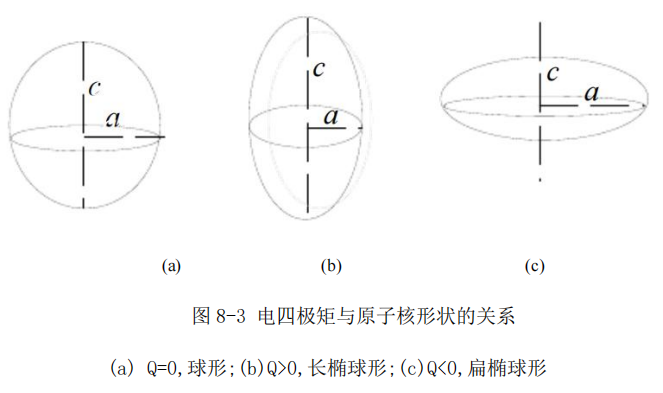
\includegraphics[scale=0.3]{t83.png}\end{center}
	\subsubsection{核与环境间的超精细相互作用}
	原子核总是处在核外环境所产生的电磁场中,它们会对核能级产生影响,这种影响被称为超精细相互作用。它主要分为电单极相互作用、电四极相互作用和磁偶极相互作用三类,这三种超精细相互作用的主要特征见下表。

	\begin{center}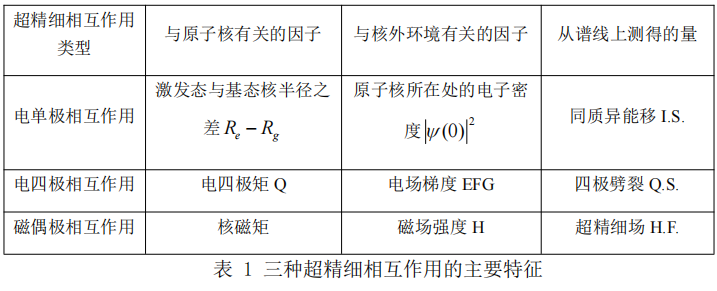
\includegraphics[scale=0.3]{b1.png}\end{center}
	1.同质异能移与电单极相互作用
	电单极相互作用是原子核的核电荷分布与核外电子密度分布之间的库仑相互作用,其作用是使核能级产生移动。其中特别是 s 电子由于其轨道的椭圆度大,在核内有一定的几率分布,核电荷和核内 s 电子云之间静电库仑作用使能级有一个微小移动E ,不同核能级对应的核体积不同,因而和 s 电子云的相互作用引起的能移不同。这些移动所引起的谱线能量的相应移动就是所谓的同质异能移。可以证明:
	\begin{equation}
	\delta=\frac{4\pi}{5}[Ze^2S(z)R^2(\frac{\triangle R}{R}][{|\psi(0)|}_a^2-{|\psi(0)|}_S^2]
	\end{equation}

	其中 S(z)是对电子密度的相对论修正,核电荷数 Z 越大,S(z)越大。R 为平均核半径,由此可以看出,同质异能移δ 不仅和激发态核半径与基态核半径之差$\triangle R$ 有关,而且还和放射源及吸收体中穆斯堡尔原子核处的电子密度之差有关。值得一提的是,${|\psi(0)|}^2$主要是指 s(1s,2s,3s,$\cdots$)电子对原子核处电子的
贡献,除 p 电子在重核的情况对此有贡献外,非 s 壳层的电子和其它近邻原子中的电子都是通过对最外层 s 电子的屏蔽作用来影响原子核处的电子密度。因此,研究同质异能移可以得到化学键性质、价态、氧化态、配位基的电负性等与核位处电子密度及电子状态有关的信息。显然这种能移与材料的化学性质密切相关的价电子相联系,所以又将它称为化学位移,由它的大小判断原子核周围价电子的分布。

	由电单极相互作用引起的核能级跃迁如图所示,它对应着穆斯堡尔图谱中的单峰:从图 8-4 中可以看出能移$\triangle E=E_0^{\prime}-E_0=\delta E_e-\delta E_g$同质异能移是一个相对参量,通常要说明是相对于何种吸收体而言。例如,$^{57}Fe$ 的同质异能移通常是以$\alpha-Fe$、$\alpha-{Fe}_2O_3$、和硝普钠(SNP)作为标准物质。

	\begin{center}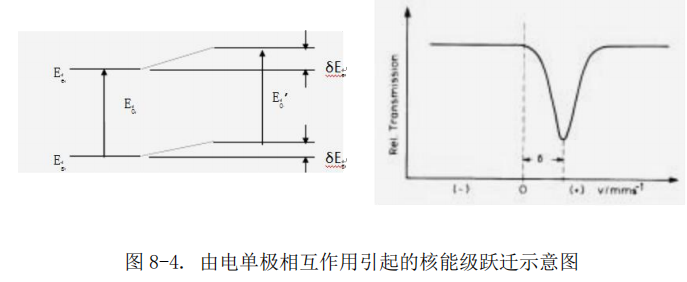
\includegraphics[scale=0.3]{t84.png}\end{center}
	2.四极劈裂与核电四极相互作用

	电四极相互作用,就是在原子核处,原子核的电四极矩与核外环境所引起的电场梯度之间的相互作用。它使能级产生细微分裂,部分消除简并,并导致谱线
的分裂。对$^{57}Fe$和$^{119}Sn$ 这两种最常用的穆斯堡尔同位素,都分裂为两条亚谱线,其间距就是四极劈裂$\triangle E_Q$。对于自旋为 I,磁量子数为$m_I$ ,电四极矩为 Q 的原子核,其四极劈裂为:
	\begin{equation}
	\triangle E_Q=\frac{e^2qQ}{2I(I-1)}[3m^2_I-I(I+1)](1+\frac{\eta^2}{3})^{\frac1 2}
	\end{equation}

	其中$eq=V_{ZZ}$是电场梯度(EFG)张量的主分量,而$\eta=\frac{V_{xx}-V_{yy} }{V_{ZZ}}$ 为 EFG 张量的不对称参量,$0\leq \eta \leq 1$。

	一般来说,原子核处的 EFG 张量有以下来源:(a)原子核周围电子云的电荷分布的不对称。例如来自满壳层的电子对的极化,或来自未充满的电子轨道上非球形对称分布的电子(b)近邻电荷。例如配位基、近邻电子。对于$^{57}Fe$ 的情形,第一类的贡献往往大于第二类贡献。而前者往往随着温度有较大的变化而后者与温度无关。通常亚谱线的强度比受到振动的各向异性、顺磁自旋驰豫、织构效应的影响,而呈现出不对称。有电四极相互作用引起的能级跃迁示意图如图 8-5 所示,它对应着穆斯堡尔图谱中的双峰:
	
	\begin{center}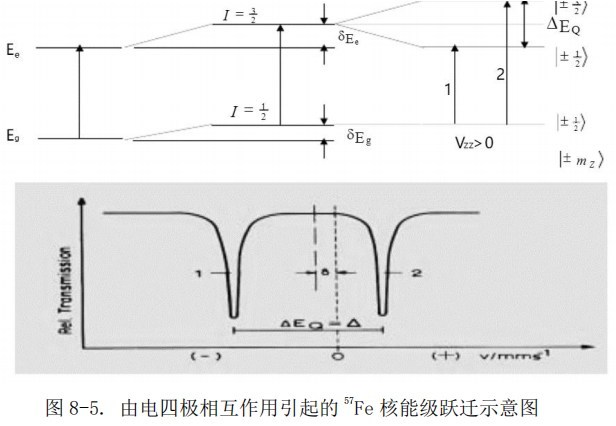
\includegraphics[scale=0.3]{t85.png}\end{center}
	简单来说,核电荷分布偏离球对称性后(I>1/2 时),相应的电四极矩与核处的电场梯度相互作用将引起能级分裂。对$^{57}Fe$ 而言,原子核的基态 I=1/2,因此电荷分布为球对称,无四极矩劈裂。而激发态 I=3/2,当$m_I$ =±1/2 时,四极矩作用使能级下移$\frac{\triangle E_q}{2}$;而当$m_I$ = ±3/2 时,四极矩作用使能级上移$\frac{\triangle E_q}{2}$;四极矩劈裂$\triangle E_q$与电四极矩$e_Q$有关,还与核处的电场梯度有关。
	
	利用四极矩劈裂可以研究形变、杂质和缺陷的影响、配位场、极化、织构等涉及共振原子核所在处局域对称性的问题。

	3.磁偶极相互作用
	
	磁偶极相互作用,即在原子核所在处原子核的磁偶极矩与核环境所引起的磁场之间的相互作用。它能使核能级产生分裂,完全消除简并。这些能级分裂,会使激发态的亚能级和基态的亚能级间发生跃迁,从而引起谱线的分裂。如图 8-6所示

	\begin{center}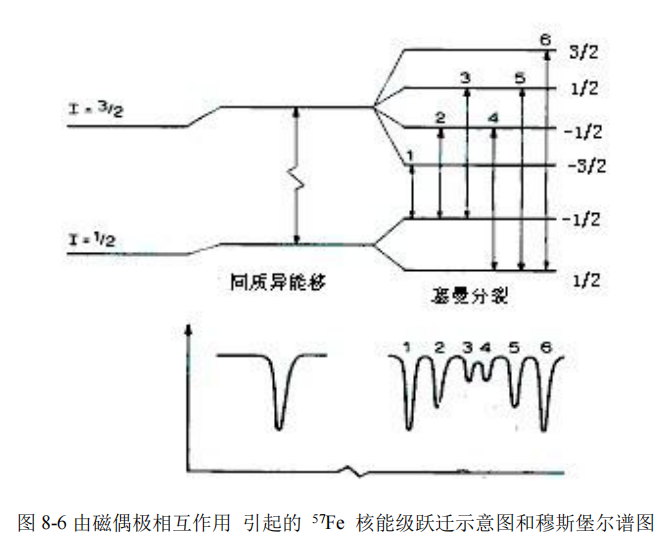
\includegraphics[scale=0.3]{t86.png}\end{center}
	这种分裂通常称为磁超精细分裂。由此可推断出原子核所在处的有效磁场$H_{eff}$。它可以是外加磁场,也可以是样品的内磁场-超精细磁场 $H_{hf}$。当不存在磁场时,原子核能级是简并的。由于核磁矩$\mu$ 与磁场 H 间存在塞曼相互作用时,核能级完全消除简并,相互作用能为:
	\begin{equation}
	E_m=-\vec{\mu}\cdot\vec{H}=-g\mu_nm_IH_{ml}\label{ci}
	\end{equation}

	其中 $\mu_n$ 为核磁子,$m_I$ 可以取-I,-I+1,$\cdots$,0,1,$\cdots$I 共有 2I+1个量子化取值,因此有 2I+1 个分裂的亚能级。对于 $^{57}Fe$ 而言,其中的基态 $I_g =\frac{1}{2}$,$g_{ng}>0$;第一激发态 $I_e=\frac{3} {2}$,$g_{ne}<0$。按照选择跃迁定则,容许的$\triangle m_I=0$、$\pm1$,因此能观察到由六个跃迁所构成的特征六线谱。实验测量得到的能级分裂大小,可以提供有关于核磁矩大小以及核处所受磁场的大小等方面的信息。六个峰的强度与γ射线前进方向和磁场方向的夹角$\theta$有关,二(五)峰与三(四)峰的强度比 x 为
	\begin{equation}
	x=\frac{4\sin^2{\theta}}{1+\cos^2{\theta}}
	\end{equation}

	$\theta = 0^{\circ}$时,$\gamma$射线方向和磁场方向平行;$\theta = 90^{\circ}$时,两者垂直。

	无反冲分数的各向异性和饱和效应都会影响谱线中各峰间的强度比。在六线谱中,一、六峰的间距正比于原子核处的超精细磁场,由此可求得超精细磁场的大小。通过磁相互作用的研究可以分辨各种磁相、测定磁转变温度、研究内磁场及其分布、极化效应、局域磁矩、驰豫效应、有序-无序转变等。这三种相互作用会单独存在,但更常见的是两种相互作用,甚至三种相互作用同时存在。如图 8-7 所示

	\begin{center}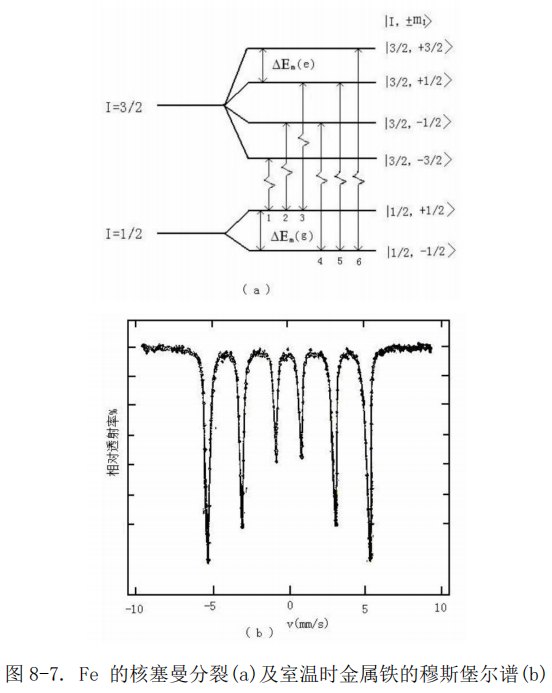
\includegraphics[scale=0.3]{t87.png}\end{center}
	从图中可以分析得到
	\begin{equation}
	\begin{cases}
	E_y\frac{V_1}{c}=\triangle E-\frac 1 2\triangle E_g-\frac 3 2\triangle E_e+\frac 1 2\triangle E_Q \\
	E_y\frac{V_2}{c}=\triangle E-\frac 1 2\triangle E_g-\frac 1 2\triangle E_e-\frac 1 2\triangle E_Q \\
	E_y\frac{V_3}{c}=\triangle E-\frac 1 2\triangle E_g+\frac 1 2\triangle E_e-\frac 1 2\triangle E_Q \\
	E_y\frac{V_4}{c}=\triangle E+\frac 1 2\triangle E_g-\frac 1 2\triangle E_e-\frac 1 2\triangle E_Q \\
	E_y\frac{V_5}{c}=\triangle E+\frac 1 2\triangle E_g+\frac 1 2\triangle E_e-\frac 1 2\triangle E_Q \\
	E_y\frac{V_6}{c}=\triangle E+\frac 1 2\triangle E_g+\frac 3 2\triangle E_e+\frac 1 2\triangle E_Q 
	\end{cases}\label{haochang}
	\end{equation}

	而同质异能移为:$\delta=\frac{c}{E_y}\triangle E$, 这样就可由上式可以求出$\delta=\frac{V_1+V_2+V_5+V_6}{4}$,$\triangle E_g=\frac{E_y}{c}(V_4-V_2)$,$\triangle E_e=\frac{E_y}{c}(V_3-V_2)$,$\triangle E_g=\frac{E_y}{c}\frac{(V_6-V_5)-(V_2-V_1)}{2}$

	\section{实验结果}
	实验中,取$v=8mm/s$,测得六个峰道址为87,159,231,284,355,427。
	由$K=\frac{10.657}{N_6-N_1}$计算出道增益为$0.0313mm/CH\cdot sec$。用此放射源测量得到的$\alpha-Fe$六线谱的位置应该在$-0.185mm/sec$的位置,所以$N_0$位置为$6+\delta$ 。
	根据$\delta = \frac{N_1+N_2+N_5+N_6}{4}$计算出实验中测量得到的$\alpha-Fe$谱的重心位置$\delta=257$,所以$$N_0=263$$

	由线性关系$v_i=(N_i-257)k$,六个峰的速度依次为-5.501 ,-3.255 ,-1.001 ,0.657 ,2.880 ,5.133 (mm/s)。由实验原理,$^{57}Fe$的能量为14.4keV,即$E_y=14.4keV$。由式\eqref{haochang}可以求得
	\begin{equation}
	\begin{aligned}
	&\triangle E = -1.61\times 10^{-8}eV\\
	&\triangle E_Q = 1.68 \times 10^{-10}eV\\
	&\triangle E_e = 1.08 \times {-7}eV\\
	&\triangle E_g = 1.88 \times 10^{-7}eV
	\end{aligned}
	\end{equation}
由式\eqref{ci}可以求得$$g_{ne}=-\frac{\triangle E_e}{\mu_n H}=-0.104$$ $$g_{ng}=\frac{\triangle E_g}{\mu_n H}=0.180$$

	实验中,谱线峰半高宽为$4204.8-3913.8=291(keV)$。由式\eqref{kd}求得第一激发态的寿命为$2.26 \times 10^{-21}$,穆斯堡尔谱的能量分辨率为$7.18\%$。

	\section{思考与讨论}
	理论上来讲,不同衬底的放射源测量出的超精细参数应该相同。因为超精细参数只与原子核和核外环境有关。不同衬底想必不至于改变电磁场分布,也不会影响到被测原子核的属性。只需要考虑发射的$\gamma$光子的一些性质,它们是可以相同的。
	应该选择自然线宽小的,反冲系数小的$\gamma$光子源,尽量选择内转换系数小,同位素多,半衰期长的。
	
	我们平常使用的$^{57}Co$放射源不可以用来测量金属$Co$样品,在室温下金属$Co$没有穆斯堡尔效应。
	也不能够测量$^{56}Fe$样品,这是因为$^{56}Fe$不是$^{57}Co$的同位素,不能吸收$^{57}Co$释放的$\gamma$射线。

	不是所有由于磁场作用产生的穆斯堡尔谱线一定是六线峰。对于$^{57}Fe$来讲,当粒子速度比较小时,就只能观察到四线峰乃至双线峰。改变被测原子后,由于核素的基态和激发态不同,所产生的峰不一定是六线。

	单道分析器选择出与穆斯堡尔效应有关的信号,将这些信号送入工作在多路定标方式的多道分析器中,此时的多道分析器的每一个道都相当于一个计数器,他们按次序记录不同时刻(相应于放射源不同的多普勒速度)到达探测器的$\gamma$光子数,每道中的计数就构成了穆斯堡尔图谱。



\end{multicols}
\end{document}